%!TEX root = ../disertace.tex
%!TEX encoding = UTF-8 Unicode

\chapter{\seman}
\label{sec:seman}
The annotation tool \seman\ is written in Perl 5\footnote{\url{www.perl.org}; \url{dev.perl.org/perl5}} with Perl/Tk\footnote{\url{http://search.cpan.org/~srezic/Tk-804.029/}} GUI toolkit. The annotation tool depends on working installation of \tred, specifically its unix installation, because it uses \texttt{nTrEd} for efficient execution of \tred\ scripts in the background. \texttt{nTrEd} however, unlike \tred\ itself or \texttt{bTrEd}, does not work on Windows.% because it uses unix sockets.

% sem-ann screenshot 
\begin{figure}[htbp]
   \centering
   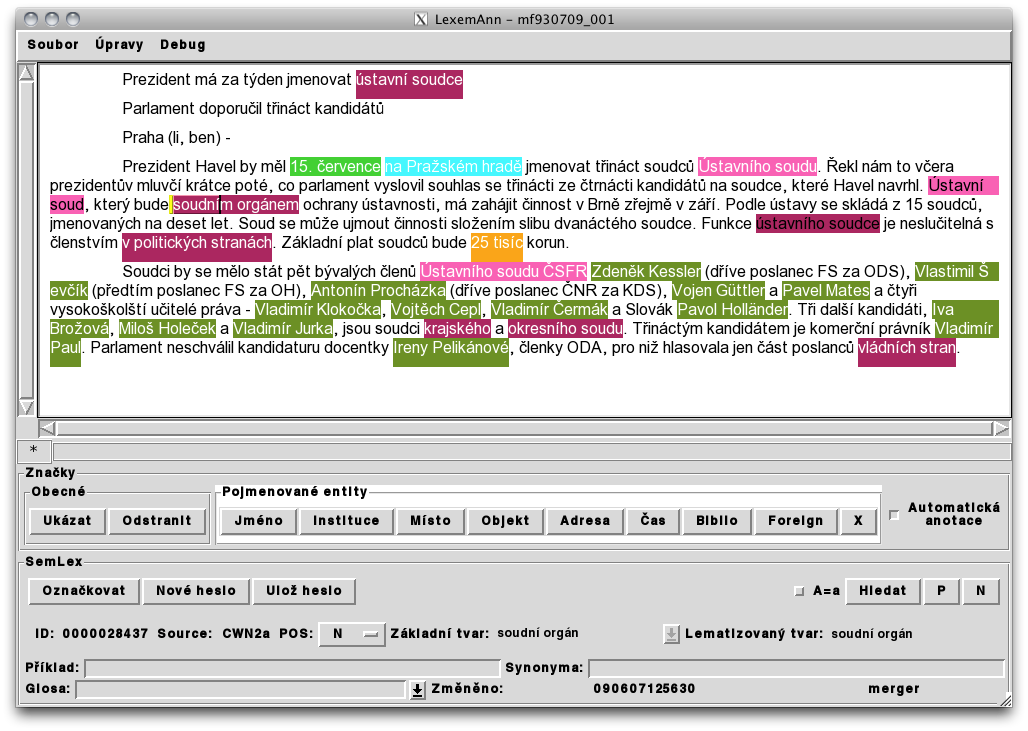
\includegraphics[width=.9\textwidth]{images/sem-ann2.png} 
   \caption{An annotated document in \seman. the yellow ``selection tag'' is barely visible on the word \pr{soudním}, because over a  different colour tag, selection has just a bezel. The \semlex\ entry that is displayed in the Semlex-part of the UI -- \pr{soudní orgán} -- is the one used to annotate the selected word. The black font colour in two tags distinguishes automatically pre-annotated MWEs.}
   \label{fig:seman-gui}
\end{figure}

\seman\ itself is composed of several main parts:
\begin{itemize}
  \item The main application file \code{sem-ann.pl} mostly implements the application frontend. It implements the GUI, loads an \sf, a \semlex,  and a log file for this \sf, if it had already been annotated. Then it takes care of all the interaction with the user and writes \sf, \semlex, and a log file.
  \item \ntred\ backend that is used to 
	\begin{itemize}
	  \item generate surface sentences from tectogrammatical trees in \tf{}s that are then displayed in the \seman\ GUI,
	  \item perform all the on-the fly pre-annotations (\Sref{sec:annot:pre})
	\end{itemize}
	What we call ``backend'' is thus the running \ntred\ instance itself (that is run by the \seman\ during start-up), and the scripts used to generate the sentences that are displayed in \seman\ and to pre-annotate MWEs using their tectogrammatical tree structures.\footnote{these scripts were written entirely by E. Bejček~(\citeyear{bejcek:2010}).}
  \item The module \code{SemLex.pm} is used to read, save, query, and edit \semlex.
    \item The module \code{SemLex\textunderscore{}heslo.pm} implements the \semlex\ entry: its structure, attributes and accessors.
  \item There is also a suite of miscellaneous scripts mostly for validation of annotated data, comparing and merging multiple annotations, merging annotators' \semlex{}es, computing reliability of annotations, and other small tasks related to annotation and managing the annotated data and \semlex{}es.
\end{itemize}

%%%%%%%%%%%%%%%%%%
\section{User interface}
\label{sec:seman:gui}
The user interface (shown in \Fref{fig:seman-gui}) is divided three main parts: The text widget displaying the annotated text, a row of buttons to create annotations by NE tags, show info on annotations, or remove tags, and an editor of \semlex. 



%%%%%%
\subsection{Text widget}
\label{sec:text-widget}
The text, displayed for the annotator, is generated from the tectogrammatical trees (using also information from lower layers). That is, why for each document to be annotated, all the PDT files must be present ( t-, a-, m-, and w-layer). 

It is possible to generate the surface (plain text) sentence from a t-tree using the `built-in' function \verb=PML_T::GetSentenceString($root)=. Such a sentence is complete, correct, has correct spacing around punctuation, but it contains no relation to the t-layer anymore. And we want to keep this connection in order to be able to annotate the t-nodes, not just words \see{sec:annot}. Thus Eduard Bejček wrote the script \url{get_sent_t-layer.btred}, that creates a representation connecting words in a sentence with tectogrammatical IDs of the t-nodes from which these words are generated. This representation is actually input into the text widget and everything but the words is hidden from the annotators' view. \emph{The tecto-IDs are then what gets really annotated, \emph{using} the words.} The full representation can, however, be displayed using Debug menu commands. It is shown in \Fref{fig:seman:hidden} in comparison to the ``plain text'' as normally displayed (with no actual annotations to keep the view simple).

%% comparison of plain text and the same with hidden text -- screenshots%%
\begin{figure}[htbp]
   \centering
   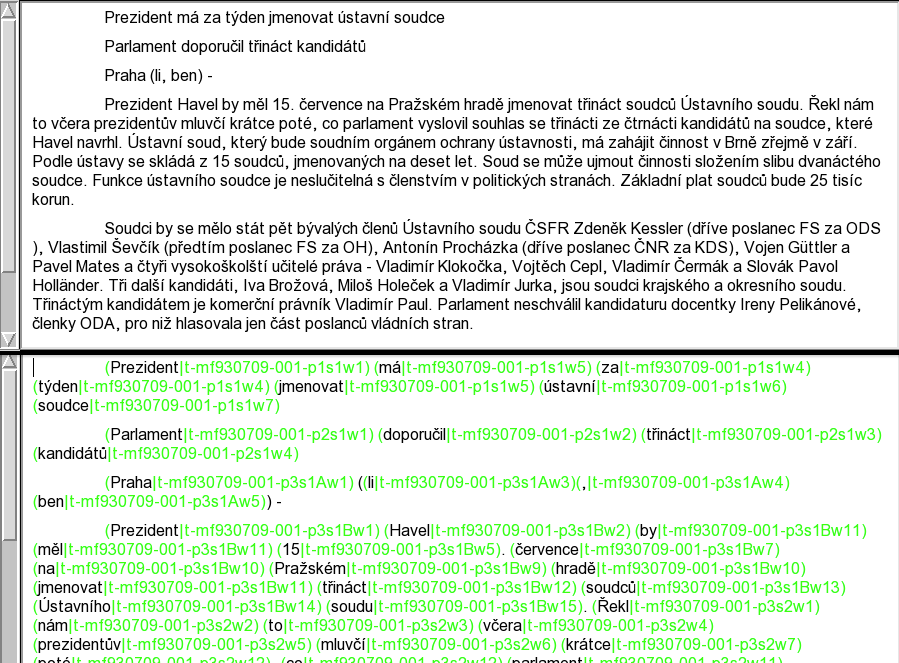
\includegraphics[width=.95\textwidth]{images/hidden-text}
   \caption{Comparison of the plain text, as normally displayed, and the underlying representation that is used to relate the actions of annotators, who mark words, to references to tectogrammatical nodes,that are actually saved in the annotation files.}
   \label{fig:seman:hidden}
\end{figure}



%%%%%%
\subsection{Annotation buttons}
The row of buttons below the text widget and the status bar is rather straightforward: 

The first group (from the left) contains two buttons that are connected to general commands used for all annotations (NEs and other \semlex\ entries alike). The first button shows a tag (i.e. the corresponding \semlex\ entry), on the word in focus (the word that is selected, or in which the cursor is placed). The second button removes the tag on the word in focus.

The second group of buttons simply creates NE tags over the selection. 

The last check button toggles the on-the-fly pre-annotation of other instances of the same MWE that annotator annotates, in the rest of the text (pre-annotation type~\ref{pre-on-annot}, see p.~\pageref{pre-on-annot}).



%%%%%%
\subsection{SemLex editor}
The \semlex\ editor and browser (see the lower part of \Fref{fig:seman-gui}) simply displays SemLex entries, allows to edit them, or to search SemLex by basic or lemmatised forms (see~\Fref{fig:semlex-search}), and browse the search results (using their basic forms). There is also a function to annotate the selected words (t-nodes) with the current SemLex entry. It is mapped simply to the return/enter key, once the focus moves from the SemLex part of the GUI to the text widget.

The attributes of an entry that are displayed include the basic and lemmatised form of an entry, its ID and source, example of usage, synonyms, if present, and a gloss. There is also a time stamp and a signature of the last modification. The attributes of a SemLex entry are explained in detail in \Sref{sec:semlex:entry}.

The search string is by default matched as a substring, and there is a check box to toggle case sensitivity. However when needed (and in case an annotator has the knowledge), full Perl regular expressions can be used. 
\begin{figure}[htbp]
   \centering
   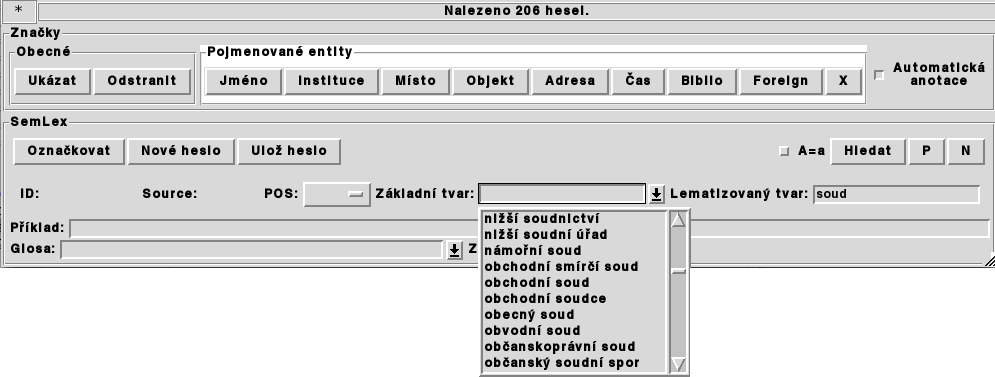
\includegraphics[width=\textwidth]{images/semlex-search}
   \caption{A result of a search in SemLex by a substring of the lemmatised form: 206 entries were found (see the status line at the top). Browsing the basic forms of the results.}
   \label{fig:semlex-search}
\end{figure}

%%%%%%
\subsection{General UI remarks}
Inspired by command mode of modal text editors and by some annotation regimes of \tred, we made all the annotation commands single-letter. That was made possible by making the text read-only. Since the letters are not used for input, they can be mapped to commands. All the command (and so the buttons) are named (in Czech) in such manner, that their first letter can be mapped to perform the command. Only the command for removing annotation is mapped to the capital letter (`O' for `odstranit') for safety reasons.


%%%%%%%%%%%%%%%%%%%
\section{Annotation logs}
\label{sec:logs}
\todo


